\documentclass[border=10pt]{standalone}
\usepackage{tikz}
\usetikzlibrary{arrows.meta,shapes,calc}

\begin{document}
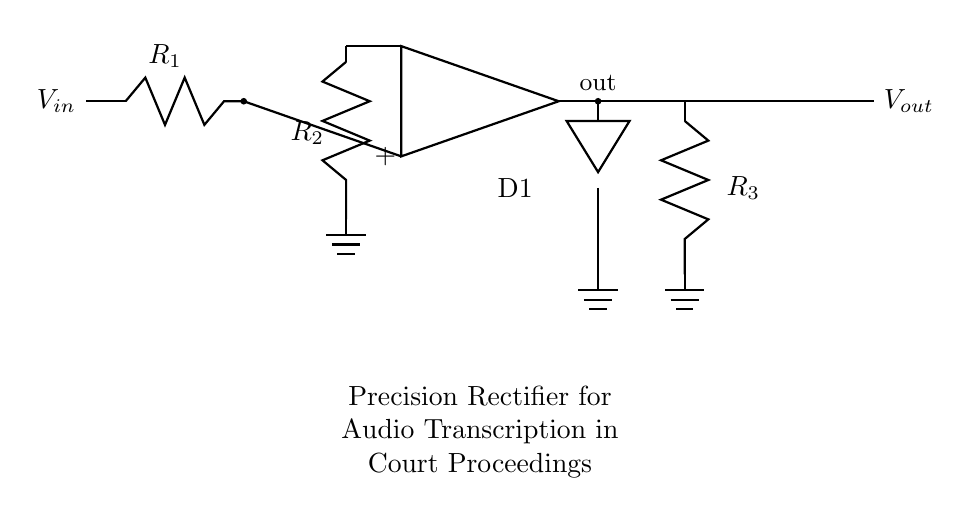
\begin{tikzpicture}[%
  >=Stealth,
  thick,
  every node/.style={font=\normalsize}
]

% Coordinates for main horizontal chain
\coordinate (Vin)   at (0,0);
\coordinate (R1R2)  at (2,0);   % junction of R1 and op-amp +
\coordinate (OP)    at (5,0);   % center of op-amp triangle
\coordinate (OUT)   at (8,0);   % op-amp output node
\coordinate (Vout)  at (10,0);  % final output label position

% Vin label
\node[left] at (Vin) {$V_{in}$};

% R1 horizontal resistor (zigzag simplified)
\draw (Vin) -- ++(0.5,0);
\draw ($(Vin)+(0.5,0)$) to[sharp corners]
      ++(0.25,0.3) -- ++(0.25,-0.6) -- ++(0.25,0.6) -- ++(0.25,-0.6)
      -- ++(0.25,0.3) -- (R1R2);
\node[above] at ($(Vin)!0.5!(R1R2)+(0,0.3)$) {$R_{1}$};

% Node at R1-opamp+
\fill (R1R2) circle (1.2pt);

% R2 vertical resistor from the negative input node to ground
\coordinate (R2top) at ($(OP)+(-1.7,0.7)$);
\coordinate (R2bottom) at ($(R2top)+(0,-2.2)$);
\draw (R2top) -- ++(0,-0.2);
\draw ($(R2top)+(0,-0.2)$) to[sharp corners]
      ++(-0.3,-0.25) -- ++(0.6,-0.25) -- ++(-0.6,-0.25)
      -- ++(0.6,-0.25) -- ++(-0.6,-0.25) -- ++(0.3,-0.25)
      -- (R2bottom);
\node[left] at ($(R2top)!0.5!(R2bottom)+(-0.15,0)$) {$R_{2}$};

% Ground symbol under R2
\draw (R2bottom) -- ++(0,-0.2) coordinate (R2g);
\draw ($(R2g)+(-0.25,0)$) -- ($(R2g)+(0.25,0)$);
\draw ($(R2g)+(-0.18,-0.12)$) -- ($(R2g)+(0.18,-0.12)$);
\draw ($(R2g)+(-0.11,-0.24)$) -- ($(R2g)+(0.11,-0.24)$);

% Op-amp triangle
\coordinate (opInMinus) at ($(OP)+(-1,0.7)$);
\coordinate (opInPlus)  at ($(OP)+(-1,-0.7)$);
\coordinate (opOut)     at ($(OP)+(1,0)$);

\draw (opInMinus) -- (opInPlus) -- (opOut) -- cycle;

% plus and minus labels
\node at ($(opInMinus)+(-0.2,0)$) {$-$};
\node at ($(opInPlus)+(-0.2,0)$) {$+$};

% input leads to op-amp
\draw (R1R2) -- (opInPlus);
\draw (opInMinus) -- (R2top); % minus input connected to R2 branch

% op-amp output
\draw (opOut) -- ++(0.5,0) coordinate (OUTA);

% Label near op-amp output "out"
\node[above] at (OUTA) {\small out};

% Output node and connection to Vout
\fill (OUTA) circle (1.2pt);
\draw (OUTA) -- (Vout);
\node[right] at (Vout) {$V_{out}$};

% Downward branch from output node
\coordinate (branchTop) at (OUTA);
\coordinate (branchBottom) at ($(branchTop)+(0,-3)$);

% Diode D1 (triangle pointing up with bar)
\coordinate (Dmid) at ($(branchTop)+(0,-1.1)$);
\coordinate (Dbot) at ($(Dmid)+(0,-1.1)$);

% vertical wire from node to diode bar
\draw (branchTop) -- ++(0,-0.25);
\draw ($(branchTop)+(0,-0.25)$) -- ++(-0.4,0) coordinate (DbarL);
\draw ($(branchTop)+(0,-0.25)$) -- ++(0.4,0) coordinate (DbarR);
\draw (DbarL) -- (DbarR); % diode bar

% triangle for diode
\draw (DbarL) -- ($(Dmid)+(0,0.2)$) -- (DbarR) -- cycle;

% vertical line from triangle tip to ground
\draw (Dmid) -- (Dbot);

% Ground under diode
\draw (Dbot) -- ++(0,-0.2) coordinate (Dg);
\draw ($(Dg)+(-0.25,0)$) -- ($(Dg)+(0.25,0)$);
\draw ($(Dg)+(-0.18,-0.12)$) -- ($(Dg)+(0.18,-0.12)$);
\draw ($(Dg)+(-0.11,-0.24)$) -- ($(Dg)+(0.11,-0.24)$);

% Diode label D1
\node[left] at ($(Dmid)+( -0.7,0)$) {D1};

% R3 vertical resistor in parallel with diode, on a separate right branch
\coordinate (R3top) at ($(branchTop)+(1.1,0)$);
\coordinate (R3bottom) at ($(R3top)+(0,-2.2)$);
\draw (branchTop) -- (R3top);

\draw (R3top) -- ++(0,-0.25);
\draw ($(R3top)+(0,-0.25)$) to[sharp corners]
      ++(0.3,-0.25) -- ++(-0.6,-0.25) -- ++(0.6,-0.25)
      -- ++(-0.6,-0.25) -- ++(0.6,-0.25) -- ++(-0.3,-0.25)
      -- (R3bottom);

% Ground under R3
\draw (R3bottom) -- ++(0,-0.2) coordinate (R3g);
\draw ($(R3g)+(-0.25,0)$) -- ($(R3g)+(0.25,0)$);
\draw ($(R3g)+(-0.18,-0.12)$) -- ($(R3g)+(0.18,-0.12)$);
\draw ($(R3g)+(-0.11,-0.24)$) -- ($(R3g)+(0.11,-0.24)$);

\node[right] at ($(R3top)!0.5!(R3bottom)+(0.4,0)$) {$R_{3}$};

% Caption text below
\node[align=center] at ($(OP)+(0,-4.2)$) {Precision Rectifier for\\
  Audio Transcription in\\
  Court Proceedings};

\end{tikzpicture}
\end{document}
